\section{Formale Definition}
\label{sec:model-definition}

Weil sie fähig sind, Zustände zu speichern, eignen sich sog. «\glspl{rnn}» (in der restlichen Arbeit wird die Abkürzung «\acrshort{acr-rnn}» verwendet) besonders gut, um Sequenzen zu lernen.
Die natürliche Sprache besteht aus Sequenzen von Wörtern, die in sich wiederum aus Buchstabensequenzen bestehen.
Deshalb kommen \acrshort{acr-rnn} bis heute in vielen Gebieten von natürlichsprachlicher Textverarbeitung zum Einsatz.

Die Besonderheit eines \acrshort{acr-rnn}'s liegt darin, dass die \glspl{neuron} – anders als bei einfachen neuronalen Netzen – nicht nur den Wert der vorangehenden Netzschicht als
Eingangswert erhalten, sondern auch den Ausgabewert des vorangehenden Zeitschritts ihrer selbst.
Jede \gls{cell} speichert den Zustand der bisherigen Zeitschritte als sog. «hidden state», der mit der Variable $ h $ gekennzeichnet wird (siehe Abb. \ref{fig:rnn-model-definition-memory-cell}).
Da das \gls{neuron} einer Art Erinnerung fähig und zudem komplexer aufgebaut ist als ihre gewöhnlichen Pendants, wird es als «Memory Cell» oder einfach als \gls{cell} bezeichnet.
Der Wert der Zellenausgabe $ y $ sowie der Zustand $ h $ werden beide durch eine Funktion $ f(h_{(t-1)}, x_{(t)})$ anhand des Zustandes aus dem vorangehenden Zeitschritt sowie der Eingabe berechnet.
Die beiden Funktionen können, müssen aber nicht den gleichen Wert ausgeben.
Für nähere Details zur Architektur, Berechnung sowie Funktionsweise sei auf die exzellente Beschreibung in \autocite{geron} verwiesen.

\begin{figure}
    \centering
    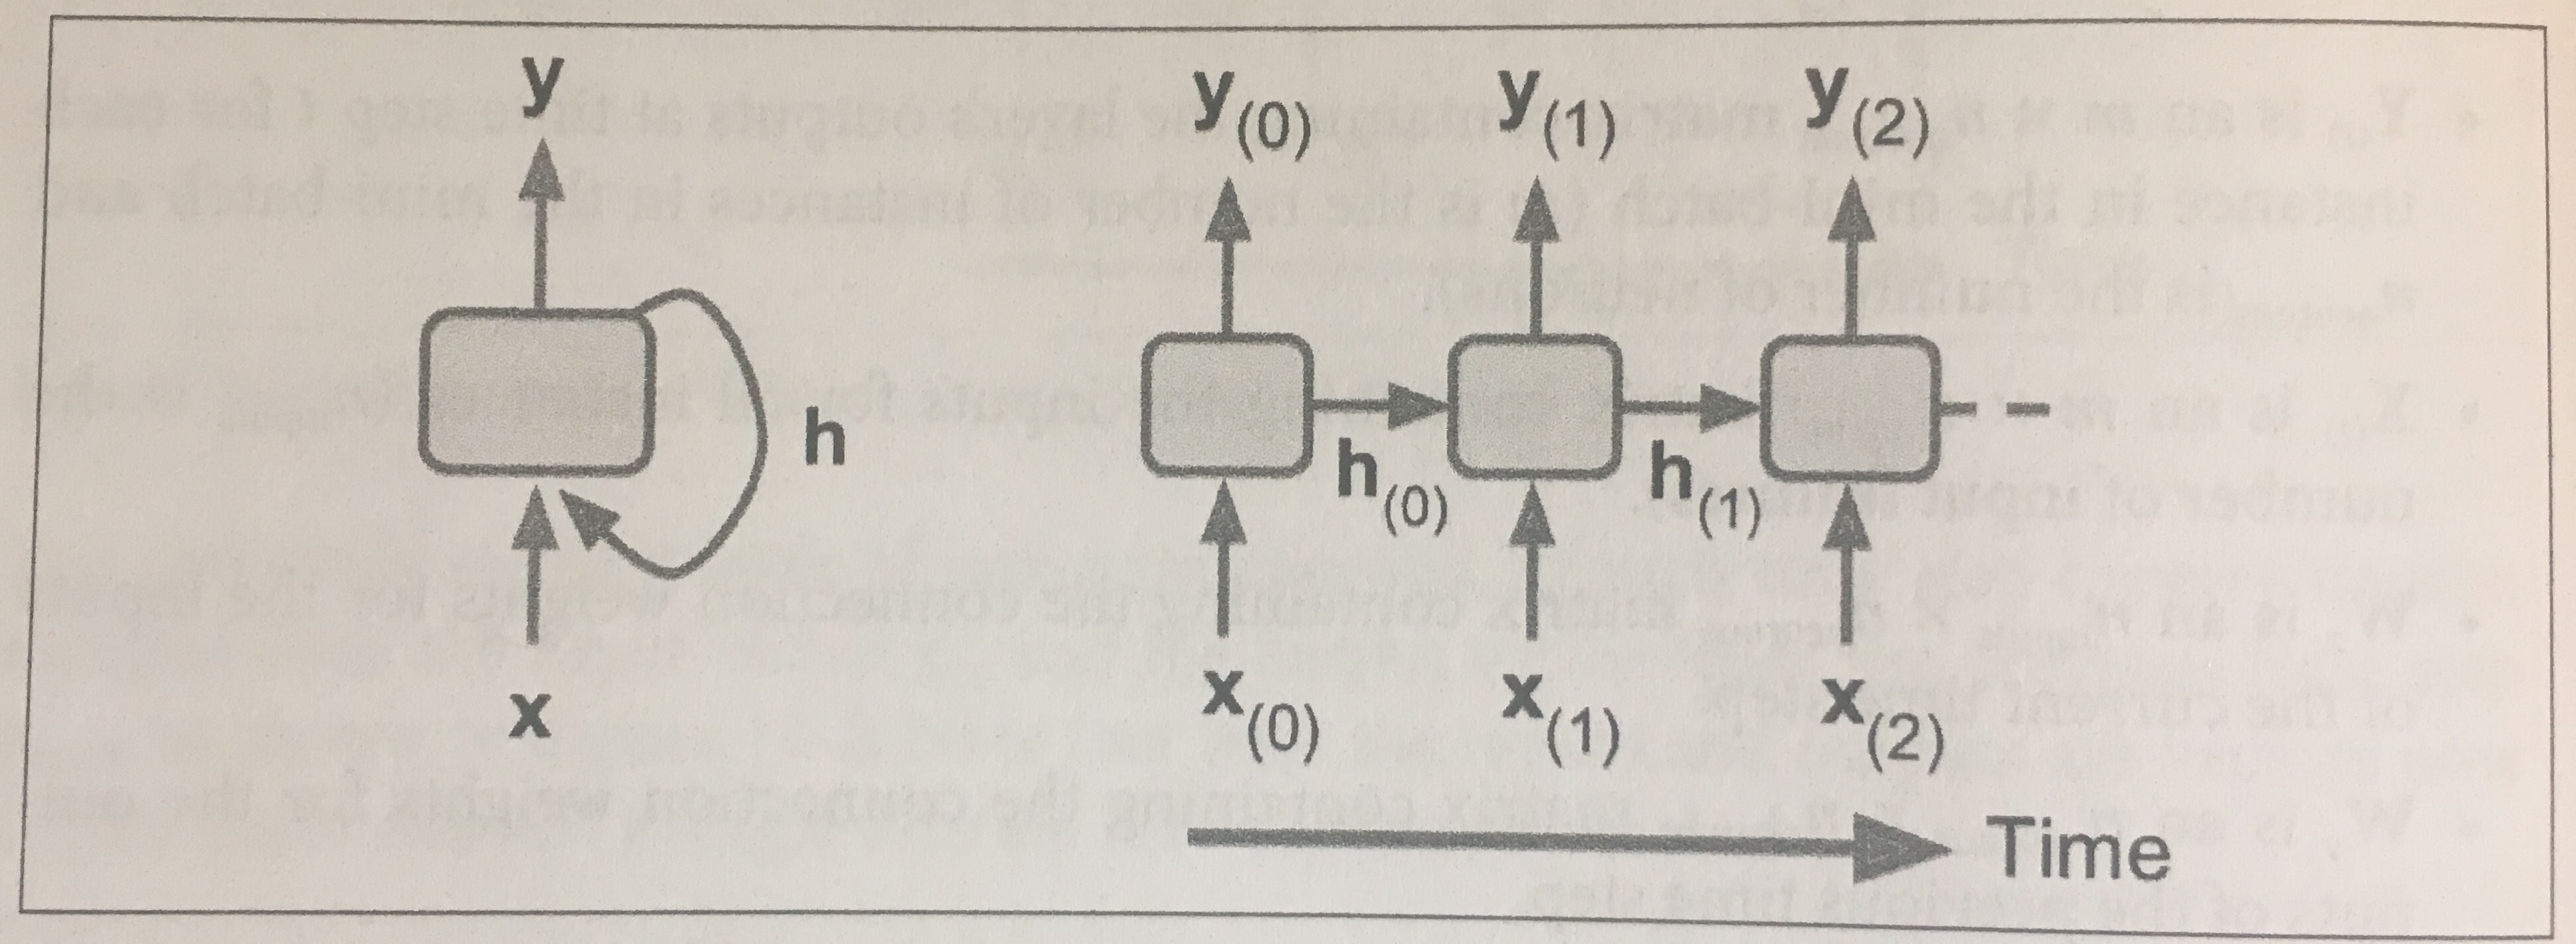
\includegraphics[width=0.75\linewidth]{images/model/model-rnn-definition.jpg}
    \caption[RNN Modell]{Memory-Zelle eines RNN \autocite{geron}. Der Zustand des vorangehenden Zeitschritts ($ h $) wird der Zelle im aktuellen Zeitschritt erneut überreicht (links).
    Das Modell wird über die Zeit «ausgerollt», wobei die Zellen jeweils den Trainingseingabevektor ($ X_{(0)} $ bis $ X_{(2)} $) sowie den Zustand ($ h_{(0)} $ bis $ h_{(1)} $) erhalten (rechts).}
    \label{fig:rnn-model-definition-memory-cell}
\end{figure}

Zwei gut bekannte Probleme, die einfache RNN-Memory-Zellen aufweisen sind einerseits das sog. «Exploding/Vanishing Gradient Problem», bei dem insbesondere in mehrschichtigen neuronalen Netzen
die propagierten Werte «explodieren» oder gegen null verschwinden, andererseits das Problem, dass anfangs eingespeiste Informationen gegen Ende der Sequenz verloren gehen \autocite{geron}.
Zur Lösung dieses Problems wurden sog. «\glspl{lstm}» (\acrshort{acr-lstm})\autocite{lstm} und später sog. «\glspl{gru}» (\acrshort{acr-gru})\autocite{gru} entwickelt.
Beide Zelltypen implementieren einen komplexen Mechanismus, der vereinfacht gesagt «unwichtiges» von «wichtigem» Wissen unterscheidet und den Lernprozess entsprechend steuert.
Weil sich beide «Gedächtniszellen» als sehr effektiv erwiesen haben, werden einfache RNN-Zellen schon fast nicht mehr verwendet.
Für das hier angewandte Modell sollen \acrshort{acr-lstm} verwendet werden.

Das Modell wird auf Basis einer konstanten Zeichenmenge $ V = \{ "a", "b", "c", ...\} $ trainiert, die das «Vokabular» beinhaltet.
Pro Trainingsschritt erhält das Modell eine Zeichensequenz der konstanten Länge $ t $, bestehend aus numerischen Zeichenrepräsentationen des Vokabulars $ V $.
Die Sequenzlänge $ t $ entspricht der Anzahl Zeitschritte, über die das Modell für jede Sequenz «ausgerollt» wird.

Die Ausgabe des Modells ist ein Vektor mit $ |V| $ Komponenten.
Für jedes Zeichen des Vokabulars $ V $ wird also aufgrund der eingegebenen Sequenz ein Wert berechnet.
Damit der Ausgabevektor des Modells für die Vorhersage des nächsten Zeichens verwendet werden kann, wird er mit der Softmax-Funktion normalisiert.
Die Softmax-Funktion ist definiert durch:

\[ \sigma(x)_{j} = \frac{e^{x}}{\sum_{k=1}^{K} e^{x_{k}}} \]

wobei $ x $ der Wert der $ j $-ten Vektorkomponente ist und $ K $ der Anzahl Vektorkomponenten entspricht.
Die Exponentialfunktion wandelt sämtliche Werte $ x $ in positive Werte um, und die Division durch die Summe aller Exponentialwerte berechnet den prozentualen Anteil jeden Wertes.
Alle Anteile bzw. Wahrscheinlichkeiten addiert ergeben wiederum $ 1 $.
Der Ausgabevektor beschreibt somit die vom Modell erlernte Wahrscheinlichkeit, nach der jedes einzelne Zeichen im Vokabular $ V $ aufgrund der eingegebenen Sequenz als nächstes Zeichen folgt.
Erhält das Modell also beispielsweise die Sequenz «Chicke», so soll der Ausgabevektor das Zeichen «n» mit der höchsten Wahrscheinlichkeit auszeichnen.
Der vom Modell errechnete Ausgabevektor $ \hat{y} $ wird mit dem Zielwert $ y $ anhand von \gls{cross-entropy} verglichen und
Abweichungen zunehmend nach logarithmischem Wachstum «bestraft»\footnote{https://ml-cheatsheet.readthedocs.io/en/latest/loss\_functions.html#cross-entropy}.
Durch \gls{backpropagation-through-time}\footnote{https://machinelearningmastery.com/gentle-introduction-backpropagation-time/} wird das Modell nach jedem Trainingsschritt im \gls{gradient-descent}
so angepasst, dass die berechnete Abweichung von $ \hat{y} $ zum Zielwert y kleiner wird.
Der Aufbau des Modells ist schematisch in Abb. \ref{fig:rnn-model-definition} beschrieben.

\begin{figure}
    \centering
    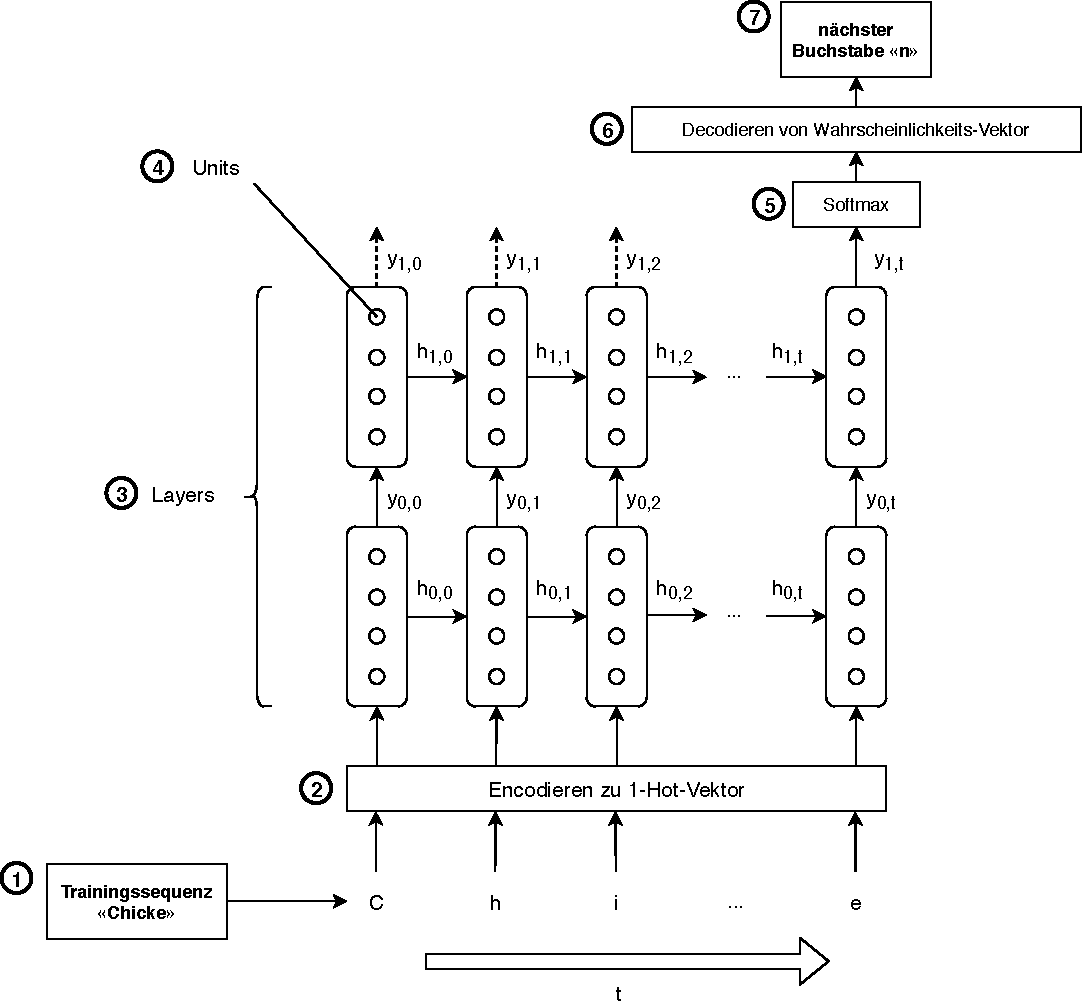
\includegraphics[width=0.9\linewidth]{images/diagrams/model.pdf}
    \caption{RNN Modell: Eine Trainingssequenz (1) wird Buchstabe um Buchstabe in das Modell eingegeben.
    Weil Buchstaben an sich nicht für arithmetische Operationen innerhalb des RNNs verwendet werden können, werden sie V-dimensionale One-hot-Vektoren encodiert, wobei die Konstante $ V $ die Menge des Vokabulars darstellt (2).
    Anschliessend wird jedem Buchstaben (also für jeden Zeitschrit) die Jahreszahl angehängt (3).
    Das RNN besteht aus einer oder mehreren Schichten (4).
    Eine RNN-Zelle besteht wiederum aus einer bestimmten Anzahl an Neuronen oder «Units» (5).
    Nachdem die ganze Buchstabensequenz ins RNN eingegeben wurde, wird der letzte Ausgabe-Vektor der LSTM-Zelle ($ y_{1,t} $) durch einen Softmax-Layer auf den Wertebereich (0.0, …, 1.0) normalisiert (6).
    So stellt der Ausgabevektor eine Wahrscheinlichkeitsverteilung über das ganze Vokabular dar.
    Der Index derjenigen Vektor-Komponente mit der höchsten Wahrscheinlichkeit ist gleichzeitig der Index des vorhergesagten nächsten Buchstanbes in der Sequenz im Vokabular.
    Mithilfe der Wahrscheinlichkeitsverteilung wird der One-Hot-Vektor zu einem Buchstaben dekodiert (7).
    Dieser Buchstabe wird dann der Sequenz angehängt (8) und der Kreislauf beginnt von vorne.}
    \label{fig:rnn-model-definition}
\end{figure}

